%% LyX 2.3.7 created this file.  For more info, see http://www.lyx.org/.
%% Do not edit unless you really know what you are doing.
\documentclass[english]{article}
\usepackage[T1]{fontenc}
\usepackage[latin9]{inputenc}
\usepackage{geometry}
\geometry{verbose,tmargin=2cm,bmargin=2cm,lmargin=3cm,rmargin=2cm,headheight=1cm,headsep=1cm,footskip=1cm}
\usepackage{amsmath}
\usepackage{amssymb}
\usepackage{graphicx}
\usepackage{setspace}
\onehalfspacing

\makeatletter
\@ifundefined{showcaptionsetup}{}{%
 \PassOptionsToPackage{caption=false}{subfig}}
\usepackage{subfig}
\makeatother

\usepackage{babel}
\begin{document}

\section{Example: Periodic Motion Planning for the Pendubot System }

\begin{figure}
\begin{centering}
\includegraphics[width=6cm]{/home/msurov/sirius/double-pendulum/fig/pendubot-schematic}
\par\end{centering}
\caption{\label{fig:pendubot-schematic} The Pendubot system.}
\end{figure}

To illustrate the main contribution of this paper, we explore the
existence of forced periodic trajectories of the Pendubot system~\cite{Spong1998}.
The system represents a two links robot with revolute joints that
moves within a vertical plane. The first joint is actuated by a DC
motor, while the second joint rotates freely. Let the generalized
coordinates $q\in\mathbb{R}^{2}$ be set as in Figure~\ref{fig:pendubot-schematic}
and let the DC motor operate in torque control mode. Then, dynamics
of the robot are written as 
\begin{equation}
M\left(q\right)\ddot{q}+C\left(q,\dot{q}\right)\dot{q}+G\left(q\right)=Bu\label{eq:pendubot-dynamics}
\end{equation}
with matrix coefficients 
\begin{align*}
 & \,M\left(q\right)=\left(\begin{array}{cc}
p_{1}+2p_{2}\cos q_{2} & p_{3}+p_{2}\cos q_{2}\\
p_{3}+p_{2}\cos q_{2} & p_{3}
\end{array}\right),\\
 & \,C\left(q,\dot{q}\right)\dot{q}=p_{2}\sin q_{2}\left(\begin{array}{c}
-2\dot{q}_{2}\dot{q}_{1}-\dot{q}_{2}^{2}\\
\dot{q}_{1}^{2}
\end{array}\right),\quad B=\left(\begin{array}{c}
1\\
0
\end{array}\right),\\
 & \,G\left(q\right)=g\left(\begin{array}{c}
-p_{4}\sin q_{1}-p_{5}\sin\left(q_{1}+q_{2}\right)\\
-p_{5}\sin\left(q_{1}+q_{2}\right)
\end{array}\right),
\end{align*}
where $g,p_{1},...,p_{5}$ are physical parameters of the robot, depending
on geometric relations and mass distribution. We set 
\begin{align*}
 & \,p_{1}=0.4\text{kg}\cdot\text{m}^{2}, & \quad & \,p_{2}=0.1\text{kg}\cdot\text{m}^{2}, & \quad & \,p_{3}=0.1\text{kg}\cdot\text{m}^{2}, & \quad\\
 & \,p_{4}=0.3\text{kg}\cdot\text{m}, & \quad & \,p_{5}=0.1\text{kg}\cdot\text{m}, & \quad & \,g=9.81\frac{\text{m}}{\text{s}^{2}}. & \,
\end{align*}

For the Pendubot, we propose identifying configuration space points,
a small neighborhood of which possesses periodic trajectories. If
we limit ourselves to the case of regular reduced dynamics, then to
solve this problem we may consider a linear servo constraint 
\[
\Phi\left(\theta\right)=q_{e}+v\theta
\]
with constants $v\in\mathbb{R}^{2}$, $q_{e}\in\mathbb{R}^{2}$. According
to Theorem~3 formulated in~\cite{Shiriaev2006} we require that
the resulting reduced dynamics exhibit a center-type equilibrium at
the point $q_{e}$. This is achieved when $q_{e}$ satisfies the equation
\begin{equation}
\gamma\left(0\right)=B_{\perp}G\left(q_{e}\right)=0\label{eq:gamma_eq_0}
\end{equation}
and there exists $v$, such that the system of inequalities
\begin{align}
 & \quad\alpha\left(0\right)=B_{\perp}M\left(q_{e}\right)v\ne0\quad\text{and}\label{eq:dgamma_ge_0}\\
 & \quad\frac{\gamma'\left(0\right)}{\alpha\left(0\right)}=\frac{B_{\perp}\left(\frac{\partial G}{\partial q}\right)_{q=q_{e}}v}{B_{\perp}M\left(q_{e}\right)v}>0\nonumber 
\end{align}
holds true. The system (\ref{eq:gamma_eq_0}, \ref{eq:dgamma_ge_0})
is written explicitly as 
\begin{align*}
\sin\left(q_{e,1}+q_{e,2}\right) & =0,\\
\cos\left(q_{e,1}+q_{e,2}\right)v_{1}+\cos\left(q_{e,1}+q_{e,2}\right)v_{2} & <0,\\
\left(p_{3}+p_{2}\cos q_{e,2}\right)v_{1}+p_{3}v_{2} & >0
\end{align*}
and it is solvable when 
\[
q_{e,1}+q_{e,2}=\pi k,\quad q_{e,1}\ne\frac{\pi}{2}+\pi n,\quad k,n\in\mathbb{Z}.
\]
As a result, we conclude that the Pendubot possesses periodic trajectories
in a vicinity of configurations where the second link of the robot
is oriented vertically, while the first link can take any position
except for the horizontal one. 

The question immediately arises: \textit{are there periodic trajectories
near other configurations of the robot?} \textit{For example, does
a periodic trajectory exist in which the robot's second link oscillates
near the horizontal position?}

To address this question, let us consider the case when the reduced
dynamics are not supposed to be regular. In this regard, we introduce
the servo constraint 

\begin{align}
\Phi\left(\theta\right) & =q_{s}+\left(\begin{array}{c}
-p_{3}\\
p_{3}+p_{2}\cos q_{2,s}
\end{array}\right)\theta+\frac{k}{2p_{3}}\left(\begin{array}{c}
0\\
1
\end{array}\right)\theta^{2},\label{eq:singular_connection}
\end{align}
where $k\in\mathbb{R},\,q_{s}\in\mathbb{R}^{2}$ are constant parameters.
If we select $B_{\perp}=\left(0,1\right)$, then the coefficients
$\alpha,\beta,\gamma$ of the reduced dynamics
\[
\alpha\left(\theta\right)\ddot{\theta}+\beta\left(\theta\right)\dot{\theta}^{2}+\gamma\left(\theta\right)=0
\]
evaluate to

\begin{align*}
\alpha\left(\theta\right) & =k\theta+p_{2}p_{3}\cos q_{s,2}-p_{2}p_{3}\cos\left(q_{s,2}+p_{3}\theta+p_{2}\theta\cos q_{s,2}+\frac{k\theta^{2}}{2p_{3}}\right),\\
\beta\left(\theta\right) & =k+p_{2}p_{3}^{2}\sin\left(p_{3}\theta+p_{2}\theta\cos q_{s,2}+q_{s,2}+\frac{k\theta^{2}}{2p_{3}}\right),\\
\gamma\left(\theta\right) & =-gp_{5}\sin\left(q_{s,1}+q_{s,2}+p_{2}\theta\cos q_{s,2}+\frac{k\theta^{2}}{2p_{3}}\right).
\end{align*}
As is readily apparent that the constraint $\Phi\left(\theta\right)$
ensures the reduced dynamics become singular at $\theta=0$, corresponing
the robot's configuration $q_{s}$. To determine whether the singular
point is permeable, we outline the conditions of Theorem~1 for its
neighborhood:
\begin{align}
\alpha'\left(0\right)=k+\frac{1}{2}p_{2}^{2}p_{3}\sin2q_{s,2}+p_{2}p_{3}^{2}\sin q_{s,2}>0 & \quad\text{and}\label{eq:inequalities_general_form}\\
\frac{\beta\left(0\right)}{\alpha'\left(0\right)}=\frac{k+p_{2}p_{3}^{2}\sin q_{s,2}}{k+\frac{1}{2}p_{2}^{2}p_{3}\sin2q_{s,2}+p_{2}p_{3}^{2}\sin q_{s,2}} & <-\frac{1}{2}\quad\text{and}\nonumber \\
\gamma\left(0\right)=-gp_{5}\sin\left(q_{s,1}+q_{s,2}\right) & >0.\nonumber 
\end{align}
We represent the conditions \ref{eq:inequalities_general_form} as
a system of linear inequalities in terms of in terms of $k$:

\begin{align*}
-p_{2}p_{3}^{2}\sin q_{s,2}-\frac{1}{2}p_{2}^{2}p_{3}\sin2q_{s,2} & <k\\
-p_{2}p_{3}^{2}\sin q_{s,2}-\frac{1}{6}p_{2}^{2}p_{3}\sin2q_{s,2} & >k\\
\sin\left(q_{s,1}+q_{s,2}\right) & <0,
\end{align*}
which directly provides the solvability set: at a given point $q_{s}$
there exists a $k$ satisfying (\ref{eq:inequalities_general_form})
iff $q_{s,2}\in\left(0,\frac{\pi}{2}\right)+\pi m$ and $q_{s,1}+q_{s,2}\in\left(-\pi,0\right)+2\pi n$,
where $n,m\in\mathbb{Z}$. 

It is easy to show that using a left annihilator of the opposite direction
$B_{\perp}=\left(0,-1\right)$ alters the signs of the coefficients
$\alpha,\beta,\gamma$ in the reduced dynamics. Consequently, the
conditions of Theorem~1 lead to a different system of inequalities

\begin{align}
-p_{2}p_{3}^{2}\sin q_{s,2}-\frac{1}{2}p_{2}^{2}p_{3}\sin2q_{s,2} & >k\label{eq:ineqs_v2}\\
-p_{2}p_{3}^{2}\sin q_{s,2}-\frac{1}{6}p_{2}^{2}p_{3}\sin2q_{s,2} & <k\nonumber \\
\sin\left(q_{s,1}+q_{s,2}\right) & >0.\nonumber 
\end{align}
In this case the solvability criteria becomes: $q_{s,2}\in\left(-\frac{\pi}{2},0\right)+\pi m$
and $q_{s,1}+q_{s,2}\in\left(0,\pi\right)+2\pi n$. As a result, we
infer that the Pendubot in a vicinity of $q_{s}$ satisfying
\begin{itemize}
\item either $q_{s,2}\in\left(0,\frac{\pi}{2}\right)+\pi k$ and $q_{s,1}+q_{s,2}\in\left(-\pi,0\right)+2\pi n$;
\item or $q_{s,2}\in\left(-\frac{\pi}{2},0\right)+\pi k$ and $q_{s,1}+q_{s,2}\in\left(0,\pi\right)+2\pi n$,
where $n,k\in\mathbb{Z}$
\end{itemize}
possesses periodic trajectories. The set of such points is shown in
Figure~\ref{fig:pendubot-conf-space}. As seen, there are configurations
where the robot's second link is oriented horizontally. Specifically,
if set $q_{s,1}=\frac{3\pi}{4}$ $q_{s,2}=-\frac{\pi}{4}$, $k=-p_{2}p_{3}^{2}\sin q_{s,2}-\frac{1}{3}p_{2}^{2}p_{3}\sin2q_{s,2}$,
then the conditions~\ref{eq:ineqs_v2} are satisfied. Numerical integration
of the corresponding reduced dynamics with initial conditions $\theta\left(0\right)=-0.02,\dot{\theta}\left(0\right)=0$
and $\theta\left(\frac{T}{2}\right)=0.02,\dot{\theta}\left(\frac{T}{2}\right)=0$
yields the phase trajectory presented in Figure~\ref{fig:pendubot-oscillates-near-horizontal}.
We also reconstruct the phase trajectory $\left(q_{*}\left(t\right),\dot{q}_{*}\left(t\right)\right)$
and control input $u_{*}\left(t\right)$ of the original system by
substituting the numerically obtained trajectory $\theta_{*}\left(t\right)$
into the expressions in~TODO. These plots are shown in Figure~\ref{fig:pendubot-oscillates-near-horizontal}.
As observed, all signals are smooth functions. It is important to
note that this trajectory could not be obtained with a regular servo
constraint. This indicates that the proposed approach uncovers a new
class of feasible trajectories.

\begin{figure}
\begin{centering}
\includegraphics[width=8cm]{/home/msurov/sirius/double-pendulum/data/configurations_with_oscillations}
\par\end{centering}
\caption{\label{fig:pendubot-conf-space}Configuration Space of the Pendubot.
The blue regions indicate the configurations where the conditions
of Theorem 1 may be satisfied with an appropriate servo constraint,
and thus, periodic trajectories exist near each of these configurations.
The brown line identifies the equilibrium points of the robot.}
\end{figure}

\begin{figure}
\subfloat[Projections of phase trajectory and control input]{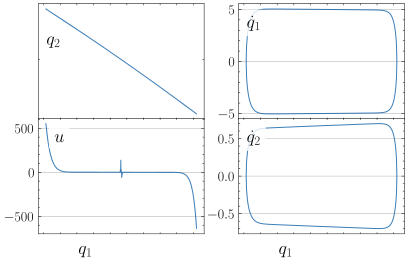
\includegraphics[width=8cm]{../data/horizontal_oscillations_trajectory}

} \subfloat[The sequence of configurations]{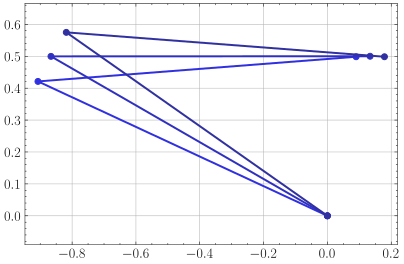
\includegraphics[width=8cm]{../data/horizontal_oscillations_schematic}

}

\caption{\label{fig:pendubot-oscillates-near-horizontal} A periodic trajectory
of the Pendubot system when its second links oscillates near horizontal
position.}
\end{figure}

\begin{figure}
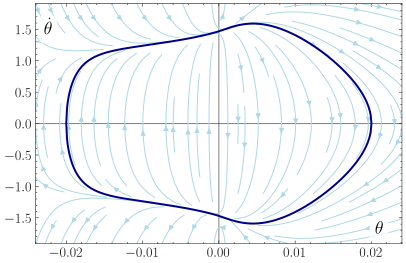
\includegraphics[width=8cm]{../data/horizontal_oscillations_phase}\caption{\label{fig:pendubot-phase-portrait} Phase portrait of the reduced
dynamics of the Pendubot.}
\end{figure}

\begin{thebibliography}{1}
\bibitem{Shiriaev2006} Shiriaev, A. and Robertsson, A. and Perram,
J. and Sandberg, A., Periodic motion planning for virtually constrained
Euler--Lagrange systems, Systems \& Control Letters, volume 55, 2006.

\bibitem{Spong1998} Spong, M.W., Underactuated Mechanical Systems,
Control Problems in Robotics and Automation, B. Siciliano and K.P.
Valavanis (Eds), Lecture Notes in Control and Information Sciences
230 Spinger-Verlag, London, UK, 1997, presented at the International
Workshop on Control Problems in Robotics and Automation: Future Directions
Hyatt Regency, San Diego, California, Dec. 1997.

\end{thebibliography}

\end{document}
